\documentclass[fontset=windows]{article}
\usepackage[]{ctex}
\usepackage[a4paper, total={6in, 10in}]{geometry}

\title{LSM的Key-Value键值对存储系统}
\author{\href{https://github.com/Musicminion}{张子谦 520111910121} }
\date{2023年 3月 14日}

\usepackage{tabularx}
\usepackage{natbib}
\usepackage{hyperref}
\usepackage{listings}
\usepackage{natbib}
\usepackage{graphicx}
\usepackage{enumitem}
\usepackage{eso-pic}


\usepackage{tikz}
\AddToHook{shipout/foreground}{
  \begin{tikzpicture}[remember picture,overlay]
    \node[black,rotate=45,scale=4,opacity=0.1] at (current page.center) {张子谦 520111910121 高级数据结构}; 
  \end{tikzpicture}
}


% \usepackage[stamp=ture]{draftwatermark}             % 所有页加水印

% \SetWatermarkText{张子谦 520111910121 高级数据结构} % 设置水印内容
% \SetWatermarkLightness{0.85}         % 设置水印透明度 0-1
% \SetWatermarkScale{0.2}             % 设置水印大小 0-1  

% \bibliographystyle{plain}

% \usepackage{xcolor}
% \usepackage[printwatermark]{xwatermark}
% \newwatermark[allpages,textcolor=gray!35,fontsize=1.5cm,textangle=60]{{张子谦 520111910121 高级数据结构}}



\begin{document}

\hypersetup{hidelinks,
	colorlinks=true,
	allcolors=black,
	pdfstartview=Fit,
	breaklinks=true
}

\maketitle

\section{背景介绍}

\subsection{历史背景}


日志结构合并树(Log Structure Merge Tree,简称LSM)在1996年由Patrick O'Neil, Edward Cheng等人提出,在计算机科学中,是一种可持久化、高效、高性能存储的数据结构。类似于其他树存储的结构,LSM会维护若干个键值对,把数据存储在内存表和持久化存储中,数据在两者之间高效地、成批地同步。

LSM树在数据库、大数据存储领域都具有非常广泛的应用。例如Apache AsterixDB/SQLite4 /InfluxDB/YugabyteDB, 以及ScyllaDB的底层存储中,都运用了这种高效的数据结构进行数据的读写操作。

\subsection{支持功能}
在这一次的课程项目中,我完成了一个简单的基于LSM Tree的键值对存储系统。支持的基本的读、写、删除操作,如下表所示。

\begin{table}[h]
  \centering
  \newcolumntype{Y}{>{\centering\arraybackslash}X}
  \makebox[\textwidth]{
  \begin{tabularx}{\linewidth}{|Y|Y|Y|}
    \hline
        操作函数 & 功能介绍 & 异常说明 \\
    \hline
        PUT(K,V) &设置键 K 的值为 V  & K存在则替换为新的V  \\
    \hline
        GET(K) &  读取键 K 的值 & K不存在则返回空字符串\\
    \hline
        DELETE(K) &  删除键 K及其对应的值 & K不存在则返回False\\
    \hline
        RESET() &  重置整个LSM系统 & 无 \\
    \hline
        SCAN(K1,K2) &  返回K1到K2直接的值 & 不要求K1/K2已存在\\ 
    \hline
  \end{tabularx}}
  \caption{实现的功能简要介绍}
\end{table}

此外,项目支持崩溃后内存数据不丢失(通过WAL,这也是数据库常见的方式),也支持范围扫描函数(SCAN)。这一部分属于附加部分的项目要求,并通过我自己的全部测试。

\subsection{项目地址}
项目代码地址:\href{https://github.com/Musicminion/2022-2023-2-Advanced-Data-Structure}{\underline{Github代码链接}}。项目时间线和提交(commit)的日志:\href{https://github.com/Musicminion/2022-2023-2-Advanced-Data-Structure/commits/main}{\underline{Commit Log链接}。}此外,在整个学期中,仓库始终保持\textbf{Private}状态,在所有的课程项目结束后,更新状态为Public。

\section{架构设计}

\subsection{架构设计前的考虑}
设计一个项目最重要的就是程序的架构。一个好的架构可以让项目更高效的推进,减少Bug的出现和修复时间。由于项目架构的确定非常重要,我一开始就反复阅读了项目需求文档,大致总结出来下面两个重要的点。(这些点忽视任何一个都可能导致项目代码大量返工)

\begin{itemize}
    \item [(1)] 
    \textbf{需要支持不同的缓存策略}。例如:内存中不缓存SSTable的任何信息、只缓存了SSTable的索引、缓存 SSTable 的 Bloom Filter 和索引。这种重要需求需要在一开始就考虑设计方式的。\textbf{如果有同学“看一页文档,写一段代码”,在开始的时候仅仅设计某一种策略,最终想要通过修改代码支持三种缓存策略,可以试想大量的代码会要重写或者覆盖,同时新的缓存策略的代码可能会对原有的代码有冲击性影响,导致程序崩溃。}
    \item [(2)] 
    \textbf{需要支持文件的二进制/文本读写} 。本项目中需要读写文件的过程非常频繁,而且需要关注不同的文件读写策略也有差异,如何设计文件读写,是整个项目最重要的地方:
    \begin{itemize}
    \item [(a)] 
    WAL(Write Ahead Log)需要支持读取(当程序崩溃之后恢复,要从WAL里面读数据)和写入(每次数据插入前都要先写到WAL)
    \item [(b)]
    SST文件的二进制读取和写入(memtable满时需要写入,程序启动时需要读)。SST的文件读写尤其重要,不仅关系到系统的正确性,还关系到后面的归并操作。
    \item [(c)]
    default.conf配置文件需要支持文本读写(启动的时候读取,当层数信息发生变化的时候需要写入)。如果只读取启动配置文件,可能导致更新的层数在下次系统启动的时候,不会读取里面的SST文件。
    \end{itemize}
\end{itemize}

其余的部分(例如归并文件的算法、SSTable索引的构建),只需要按照文档的要求编写即可正确的完成对应的功能。

\subsection{架构设计思路}

这一部分我想介绍我自己设计项目时候遇到的问题和求解思路。因为我看到身边有同学对于项目的架构设计非常困惑,在面临一个较大项目的时候,经常会纠结。项目说明文档和代码模板没有给出任何底层设计上限制或者提示,增加了自由度的同时也加大了难度。毕竟项目架构设计有非常多方法,但是最优的往往只有少数几种。

\subsubsection{错误的设计思路}
我最初采用的架构设计是\textbf{自顶向下},也就是说设计完跳表之后,我就直接开始考虑kv-store代码的编写,进而引入了Memtable和SStable两个类。但是我在接下来的设计中发现:我常常是\textbf{上层的代码需要支持一个功能的时候,就在下层的代码里面增加对应接口},这种设计时非常糟糕的。最终SStable的接口混乱不堪。加上我把所有的sst数据都放在sstable这个类,增删改查操作函数、刷新缓存策略函数、文件读写函数等各种操作直接让接口数量爆炸式增加,这样下去调试出现问题,debug更是难上加难。

SStable需要维护四个类的数据(Header数据、BF过滤器、Index索引数据、Value数据值),这些操作全部由SStable类的函数实现,会让复杂度成倍递增,而且\textbf{项目要求需要支持不同的缓存策略,后续需要分别测试},这样下来缓存刷新又需要更新类里面的容器数据,而且不同的缓存策略在SStable读取/查找数据的时候,又要分情况考虑。于是乎我果断抛弃了这种设计(当然还有大量已经写好了的代码),既然一个类复杂度太高,那我就果断\textbf{选择拆分},采用分层策略。

\subsubsection{修正的设计思路}
SStable的设计我选择拆分成四个子类组件(Header数据、BF过滤器、Index索引数据、Value数据值),SStable内部的数据只需要存储这四个类的指针,当我需要刷新缓存策略的时候(比如写完文件之后,删除BF缓存/Index缓存的时候,只需要delete指针即可,大大的简化操作。之后需要的时候构造一个即可)

接下来就面临数据读写的问题,例如sst文件读写是该在哪一层呢,顶层KVstore?还是SSTable?还是底层SStable的四个组件?最终我果断选择了SStable的组件(也就是在底层读写文件),这是因为底层的数据结构更加简单,这样也更加\textbf{便于测试},完成每一个小组件之后立刻测试。此外当我需要写入一个SStable文件的时候,只需要在上层SStable类里面依次调用下层的Header、BF过滤器、Index索引、Value数据值的写文件函数,即可完成写入。也让代码大大简化,逻辑更加清晰。

所以综上所述,正确的设计思路应该是\textbf{自底向上},编写好底层的代码(跳表、SSTable的四个组件),编写完成后立即测试(例如跳表的插入、四个组件的二进制文件读写),然后实现SStable,MemTable类,对于这些子类进行封装和维护,这样才是最佳的选择。而不是到了最终设计完成之后再测试,否则出现了问题定位极其困难。

\subsubsection{设计架构}
当我拿到这个kv-store项目需求的时候,首先分析大体架构,显然是需要包括一个内存表类和一个对应sst文件类,绘图如下:



\begin{figure}[h!]
  \centering
  \includegraphics[width=0.60\textwidth]{Image/Basic-Structure.png}
  \caption{Basic-Structure}
  \label{fig:Basic-Structure}
\end{figure}


然后基于我在前文2.2.1-2.2.2所叙述试错的经验,进一步完善设计,得到详细的架构图(参见图2)。关于架构图的具体说明如下:

\begin{itemize}
    \item [(1)] 
    第一层主要是KV-Store控制平面。是整个项目对外的接口API,提供增加、删除、修改、重置、扫描键值对范围的接口,会将不同的操作经过处理后移交到下层处理。
    \item [(2)] 
    第二层主要包括MemTable和SStable两个类。
    \begin{itemize}
    \item [(a)] 
    MemTable存储维护内存里面的Key-Value对,是对于跳表的二次封装,并记录当前跳表转化为SST文件的大小,对外暴露插入前检查函数、插入函数。
    \item [(b)]
    SStable是负责对于sst文件的文件读写、查找操作、缓存管理、元数据存储。
    \end{itemize}
    \item [(3)] 
    第三层主要是上层类的组件工具。例如MemTable底层是跳表实现的。SStable内部包含四个类(Header、BF过滤器、Index、Data)类。这四个类具有独立的文件读写功能,通过暴露写文件的接口,实现对sst的文件读写。
\end{itemize}


\begin{figure}[h!]
  \centering
  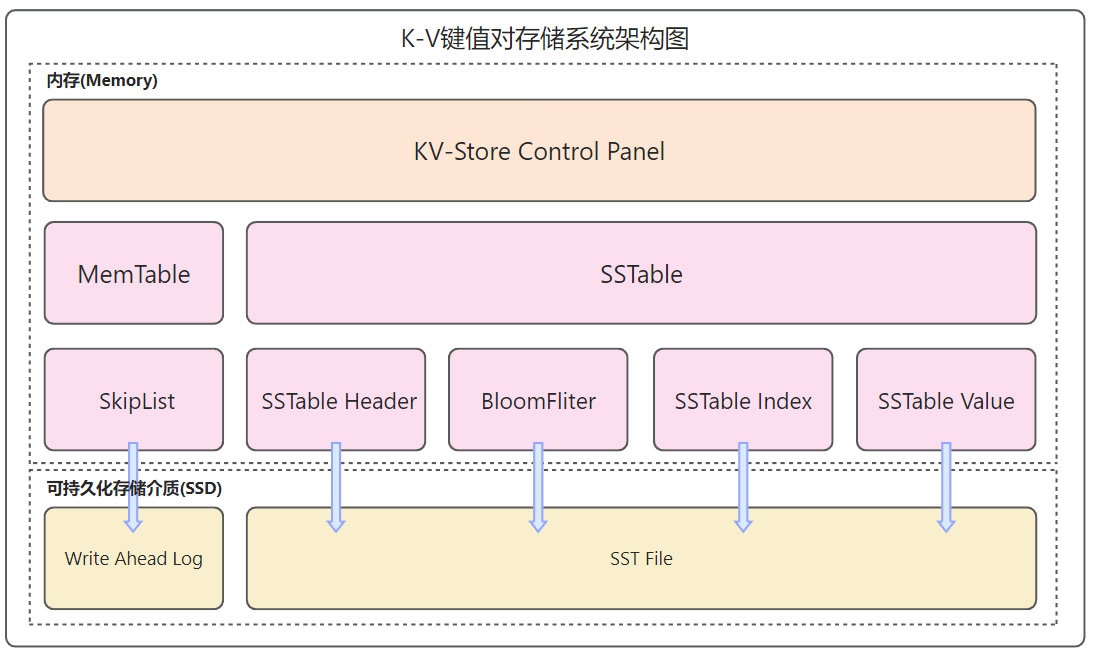
\includegraphics[width=0.98\textwidth]{Image/LSM-Architecture.png}
  \caption{KVstore-Architecture}
  \label{fig:LSM-Structure}
\end{figure}

\subsubsection{设计原则}
整个项目在设计的时候遵循下面的软件工程原则:

\begin{itemize}
    \item [(1)] \textbf{高内聚、低耦合}:以SStable下层的四个子组件为例,每个子组件功能专一,只负责读取文件的特定部分,且具有独立的读写sst文件的能力。同层级之间不存在任何相互依赖、调用关系。
    \item [(2)] \textbf{分层架构}:下层为上层提供接口,上层只需要调用对应的接口完成相关的业务逻辑。尽管分层架构在效率上有所折扣,但是代码的可维护性大大增强,可以非常快的定位到问题的根源。
    \item [(3)] \textbf{接口单一职责原则}:精简API,不暴露任何冗余接口。对于操作函数,对外暴露的会写日志,对于内部的私有函数不写日志,提供崩溃时恢复的功能。
\end{itemize}


\section{测试}
项目原始给出的测试程序仅仅测试了在顺序插入Key的范围是0到 MAX,Value为i+1个相同字母(s或者t)的时候,程序的各种状态是否能保证正确。即使是持久性测试,在测试结束之后,还插入了大量数据用于把内存部分的数据冲出到sst文件中。这种测试显然具有偶然性。

于是,为了保证项目的稳定性、鲁棒性、数据持久化,我编写了自己的测试代码。增加了数据随机化测试、数据压力测试、崩溃性测试。确保系统即使在正常运行时突然崩溃,数据量巨大等情况下,也能稳定运行。


\subsection{多进程持久性测试原理}
\textbf{提示}:由于我完成了Write Ahead Log 的部分,此部分仅仅适用于WAL已经完成的前提下测试。编写测试代码的原理如下:

首先,测试之前需要使用随机化函数,准备好数据集合。(包括Key和随机化长度随机化内容的Value),比较合适是用Map存储。

然后,基于我ICS课程所学到的,我选择fork出一个子进程,来执行程序。由于Fork出的子进程会继承fork之前父进程的内存数据空间,之后子进程执行写入我们刚刚准备好的数据集合,父进程进入等待状态。

为了验证崩溃之后是否具有数据可持久化,可以在子进程里面插入意外的崩溃事件(例如发生除0错误,操作系统会发出signal信号终止程序),程序会不经过运行时对象的析构函数,直接退出。退出之后,父进程继续进行。

最后,父进程创建kvstore对象,继续进行查找操作,验证刚刚的插入数据是否有效。


\subsection{性能测试}

\subsubsection{理论时间复杂度}

在正式测试之前,基于跳表数据结构、BF过滤器的相关理论知识,我对于设计出来的KV-Store的三种常见操作的时间复杂度做了如下评估:

\begin{itemize}
    \item [1)] \textbf{GET(K,V)}:查找的操作的时间复杂度应该分为两组情况:内存中查找、存储中查找。
    \begin{itemize}
    \item [a)] \textbf{内存查找:}使用跳表存储Key-Value对,单次查找操作的平均时间复杂度为 O(log n)。
    \item [b)] \textbf{持久化存储中查找:}首先会读取文件,然后根据布隆过滤器,由于是通过Hash函数的计算,仅需 O(1) 的时间复杂度即可判断是否在该 SSTable 中。判定存在后使用二分查找找到 offset,查找的时间复杂度为 O(log n)。
    
    \item [c)] \textbf{综合考虑:}尽管两者看上去都是O(log n)的时间复杂度,但是由于硬盘读写速度远小于内存读写速度,因此对于访问硬盘的 Get 操作,时间复杂度应该是偏大O(log n)的。
    \end{itemize}
    
    \item [2)] \textbf{PUT(K,V)}:插入的操作也应该分为两组情况:不发生归并、发生归并。
    \begin{itemize}
    \item [a)] \textbf{不发生归并:}如果不发生归并,仅在跳表中插入该键值对。跳表插入的时候首先要找到对应的节点,然后更新前面节点不同楼层对应的最近节点。时间复杂度为O(log n+K),其中K为楼层数量,由于最大楼层是个常数,所以时间复杂度为O(log n)
    
    \item [b)] \textbf{发生归并:}如果需要归并,归并消耗的时间,这数据的分布有很大的关系。归并是最消耗时间的一个步骤,因为它涉及到大量的文件读写、删除、内存排序。此外,由于我们项目要求的是删除标记用特定字符串存储,所以导致旧的废弃数据也会被归并,占用时间。
    
    但是我们可以做一个假设然后计算大概值,假设每个文件的键值对数量相仿,都为K,n为整个系统的键值对数量,楼层level的数量为L,每层里面的sst文件全部装填满。归并的时候选择时间戳较小的多出楼层限制数量的sst文件
    
    那么SST文件的个数大概就是(忽略内存表的键值对):
    $$sstFileNum = \frac{n}{K} $$
    
    然后,当有一个新的文件插入,第1层(level-0)的sst文件数量变为3,后续第i层sst文件数量为$2^i$。首先归并第一层和第二层,需要进行归并排序,归并后所有数据放在第二层,时间复杂度为:
    $$(3 + 4) \times \frac{n}{K} = (3 + 2^2)\times \frac{n}{K} $$
    于是,这7个文件放入第二层。后面进行归并第2层和第3层的时候,需要把第二层多出来的文件(第二层最多放4个文件,所以要拿出来3个)拿出来,和第三层的8个文件归并,时间复杂度为:
    $$(3 + 8) \times \frac{n}{K} = (3 + 2^3)\times \frac{n}{K} $$
    数学归纳法,得出归并第 $X$ 层和第 $X + 1$ 层的时候,需要的时间复杂度是:
    $$(3 + 2^{X+1}) \times \frac{n}{K} $$
    
    求和计算所有的归并时间:
    $$\sum_{j = 1}^{j= L} (3 + 2^{j+1}) \times \frac{n}{K} = [3L + 4(2^L - 1)] \times \frac{n}{K}$$
    
    此外,给予假设,楼层的数量$L$和sst文件的数量也存在关系:
    $$ sstFileNum = \frac{n}{K} = \sum_{i=1}^{L}2^i = 2^{L+1} - 2 $$
    
    再次计算所有的归并时间,可以有:
    $$[3L + 4(2^L - 1)] \times \frac{n}{K} = (2\frac{n}{K} +3log_2(\frac{n}{K} + 2) - 3) \times \frac{n}{K} $$
    
    所以最糟糕的时间复杂度可能高达$O(n^2)$
    \end{itemize}
    
    \item [3)] \textbf{DEL(K,V)}:删除的操作会经过查找和插入两个过程,如果查找失败,就插入一个特定的DELETE字符,所以可以认为是插入和查找(内存+持久化存储)的时间复杂度之和。但是由于插入的数据非常小,归并发生的可能也及其小,所以可以近似认为,时间复杂度为跳表插入复杂度 $O(log(n))$ + 查找时间复杂度$O(log(n))$ 的和,即为 $O(log(n))$
    

\end{itemize}


\subsubsection{操作延迟和数据量的关系}

数据量是键值对存储系统中,存储key-value对的数量。在研究操作延迟和数据量关系时,我选择固定Value的字符串长度为1024Byte,Key和Value的内容全部随机生成。测试的数据量依次是:128、256、512、1024、2048、4096、8192、16384。测试过程是依次对于生成的数据\textbf{依次}执行\textbf{插入}、\textbf{查找}、\textbf{删除},统计所有生成的数据的插入、查找、删除操作的\textbf{平均时延},统计到的测试结果如下表所示,基于该表的数据,绘制折线图:

我在选择数据的时候,恰恰选择了一个\textbf{临界点}、那就是插入的数据刚好从内存表过渡到sst文件的那个过程,因此这些图里面出现了一个\textbf{突跃}的现象。可以看到插入和删除的时延在从1024过渡到2048的时候,一下子增加了几倍。这也恰恰说明了内存的读写速度和文件的读写速度的差异。

\begin{table}[h]
  \centering
  \newcolumntype{Y}{>{\centering\arraybackslash}X}
  \makebox[\textwidth]{
  \begin{tabularx}{\linewidth}{|Y|Y|Y|Y|}
    \hline
        数据量 & PUT(s)  &  GET(s) & DEL(s)  \\
    \hline
    128 & $3.915 \times 10^{-5}$ & $4.062 \times 10^{-7}$ & $2.174 \times 10^{-5}$ \\
    \hline
    256 & $3.693 \times 10^{-5}$ & $4.648 \times 10^{-7}$ & $2.625 \times 10^{-5}$ \\
    \hline
    512 & $4.109 \times 10^{-5}$ & $5.000 \times 10^{-7}$ & $2.496 \times 10^{-5}$ \\
    \hline
    1024 & $3.658 \times 10^{-5}$ & $5.361 \times 10^{-7}$ & $2.474 \times 10^{-5}$ \\
    \hline
    2048 & $4.357 \times 10^{-5}$ & $7.883 \times 10^{-5}$ & $1.211 \times 10^{-4}$ \\
    \hline
    4096 & $4.261 \times 10^{-5}$ & $9.322 \times 10^{-5}$ & $1.280 \times 10^{-4}$ \\
    \hline
    8192 & $9.697 \times 10^{-5}$ & $1.079 \times 10^{-4}$ & $1.469 \times 10^{-4}$ \\
    \hline
    16384 & $1.091 \times 10^{-4}$ & $1.293 \times 10^{-4}$ & $1.881 \times 10^{-4}$ \\
    \hline
  \end{tabularx}}
  \caption{操作延迟和数据量关系}
\end{table}

为了验证这个临界点是否正确,我做出了如下的计算过程,当插入的数据量为1024的时候,数据Key的大小为12288Byte,Value的大小为$1024 \times 1024$,对应1MB,显然这时候是没有超过内存表的大小限制的。但是当插入的数据量为2048,Value的大小就已经达到了2MB,超过限制,所以触发了写文件操作。

\begin{figure}[h!]
  \centering
  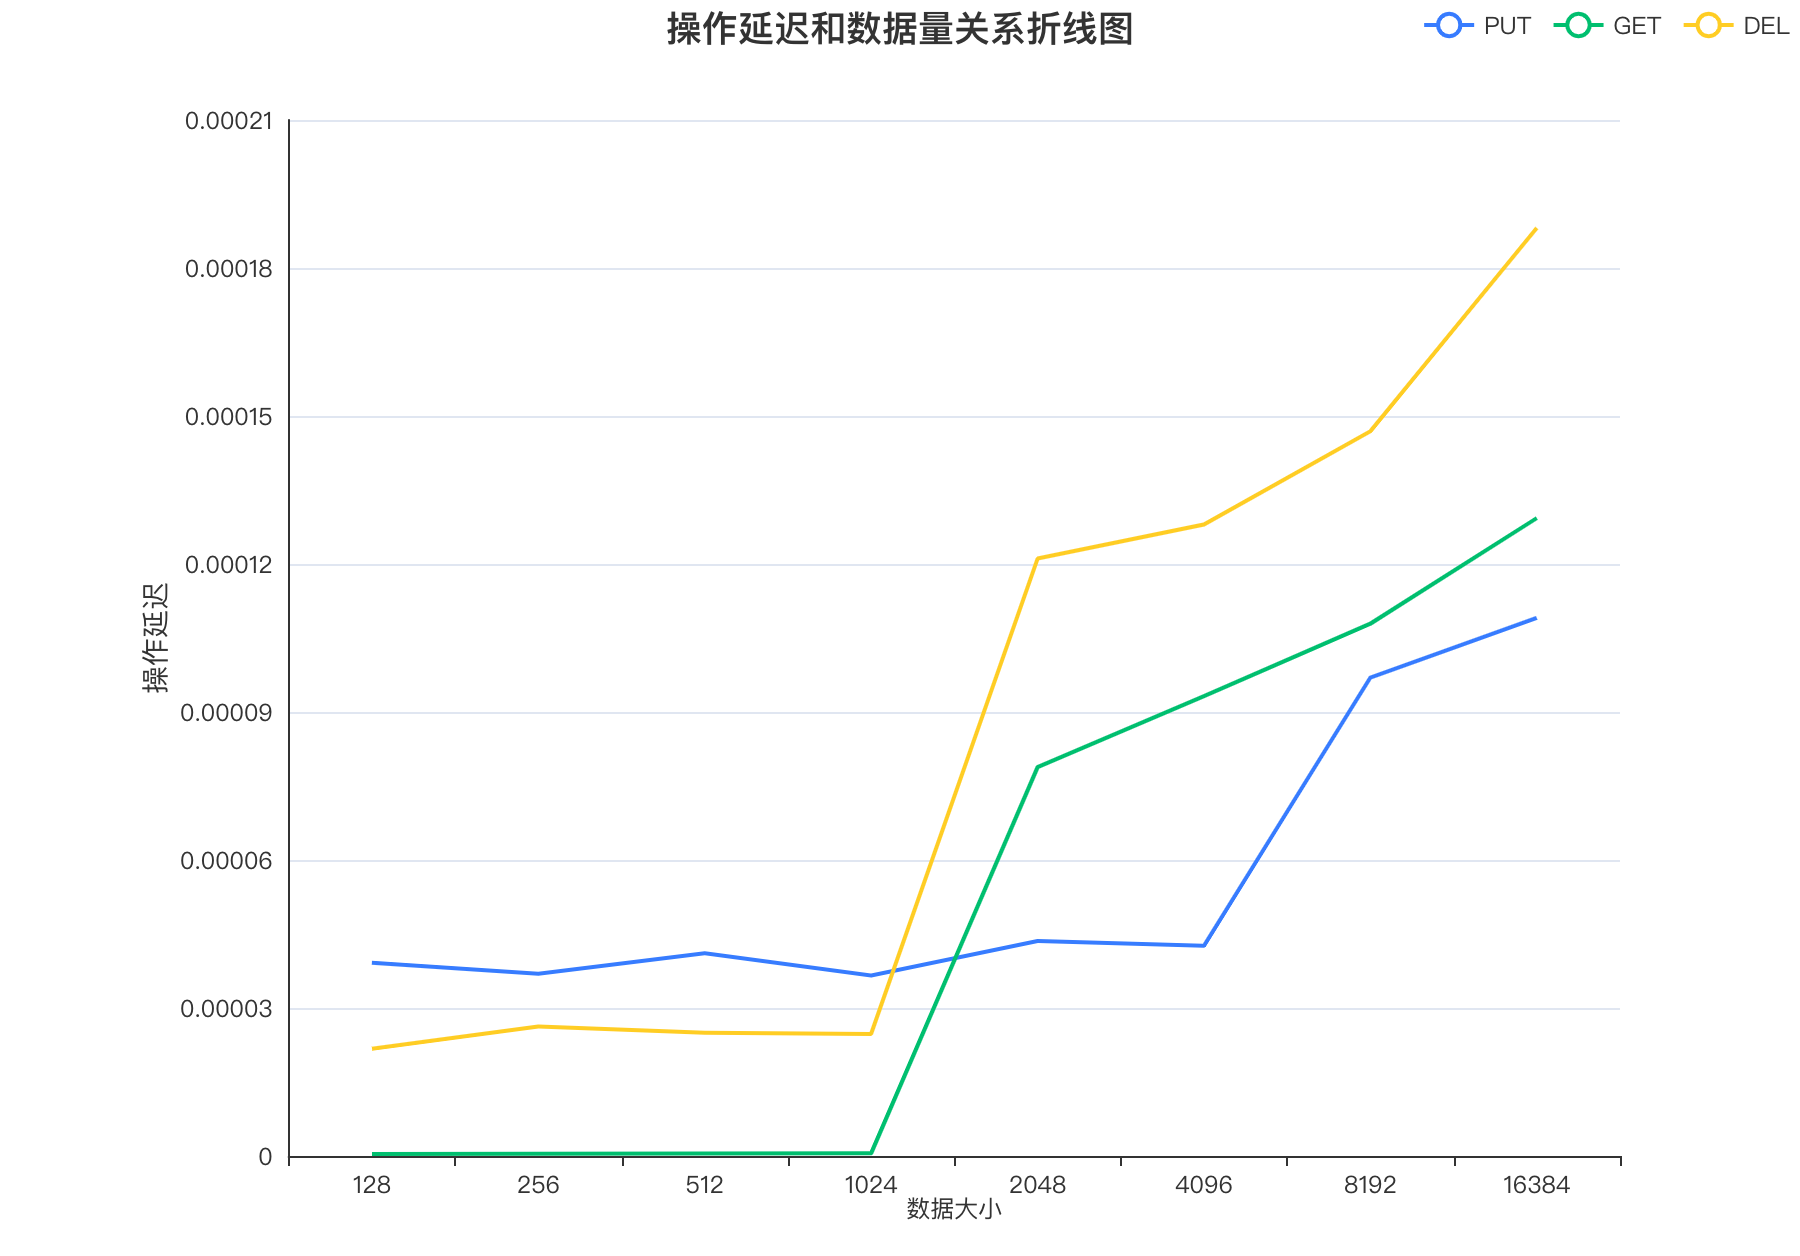
\includegraphics[width=0.98\textwidth]{Image/操作延迟和数据量关系折线图.png}
  \caption{操作延迟和数据量关系折线图}
  \label{fig:操作延迟和数据量关系折线图}
\end{figure}

那么为什么只有两根线出现了突跃现象呢?因为GET和DEL操作本质都经过了\textbf{查找}的过程,都是经过内存查找、sst文件查找(这个占主要的时间)。而PUT操作基本上就是直接在内存表里面插入数据,偶尔可能出现merge的问题,所以可以看到PUT的线增长的比较缓慢。这也是完全符合预期的!


\subsubsection{Value大小和吞吐量的关系}

根据设定,插入的Key是64位无符号整数,value作为字符串变化的空间很大。那么我也探究了Value的大小和吞吐量的关系,吞吐量是时延的倒数,代表每一秒可以插入的数据量。我在测试的时候插入的数据量为8096个($1024  \times 8$)。

\begin{table}[h]
  \centering
  \newcolumntype{Y}{>{\centering\arraybackslash}X}
  \makebox[\textwidth]{
  \begin{tabularx}{\linewidth}{|Y|Y|Y|Y|}
    \hline
        Value大小(Byte) & PUT(s)  &  GET(s) & DEL(s)  \\
    \hline
    128 & $2.2753\times 10^{4}$ & $1.2919\times 10^{6}$ & $3.5973\times 10^{4}$ \\
    \hline
    256 & $2.4298\times 10^{4}$ & $1.4636\times 10^{4}$ & $8.8935\times 10^{3}$ \\
    \hline
    512 & $2.4012\times 10^{4}$ & $1.1463\times 10^{4}$ & $7.5389\times 10^{3}$ \\
    \hline
    1024 & $1.0805\times 10^{4}$ & $9.5342\times 10^{3}$ & $6.9998\times 10^{3}$ \\
    \hline
    2048 & $8.3339\times 10^{3}$ & $7.4109\times 10^{3}$ & $5.5418\times 10^{3}$ \\
    \hline
    4096 & $4.5567\times 10^{3}$ & $4.6497\times 10^{3}$ & $3.6477\times 10^{3}$ \\
    \hline
    8192 & $2.4900\times 10^{3}$ & $2.7527\times 10^{3}$ & $2.4196\times 10^{3}$ \\
    \hline
    16384 & $1.4493\times 10^{3}$ & $1.4388\times 10^{3}$ & $1.3135\times 10^{3}$ \\
    \hline
  \end{tabularx}}
  \caption{吞吐量和Value大小的关系}
\end{table}

根据测量的时间数据,绘制折线图。由于如果把所有的范围都放在一张图中,可能会带来观察困难,所以我把图分成了两张,全局部分展示所有的数据,部分仅仅展示Value大小为256到更大的数据范围。下面我们来分析原因。



\begin{figure}[h!]
  \centering
  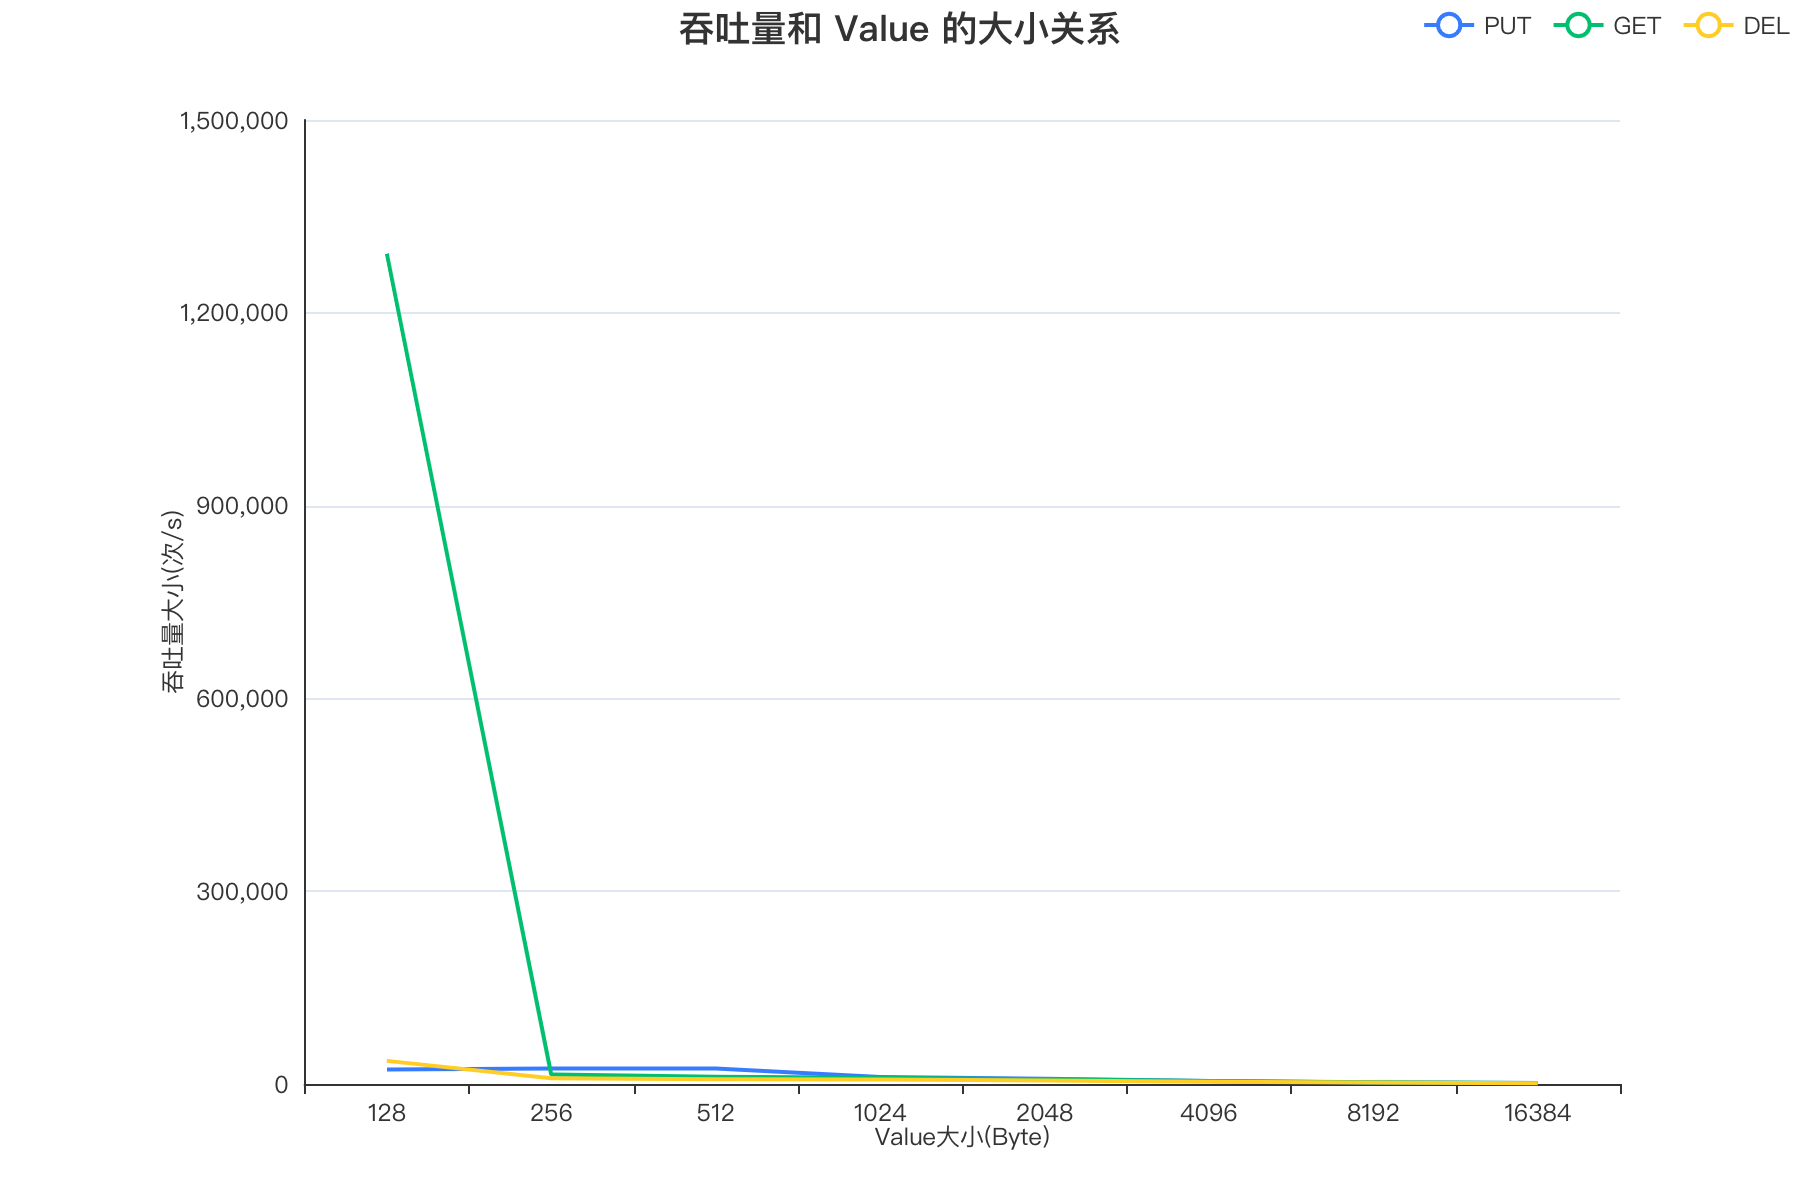
\includegraphics[width=0.98\textwidth]{Image/吞吐量和 Value 的大小关系 (全局).png}
  \caption{吞吐量和 Value 的大小关系(全局)}
  \label{fig:吞吐量和 Value 的大小关系(全局)}
\end{figure}

GET的吞吐量陡然下降的原因和之前解释的一样,就是因为从内存读写变成了文件读写,但是这里另外一个问题出现:为什么GET的吞吐量和PUT/DEL的吞吐量这么大的差别,目前推测是因为我的PUT/DEL需要写WAL日志,写文件的方式占用了时间,所以带来了差异(实际我也测试了关闭WAL,吞吐量会提高很多,由于篇幅这里就不展示附加功能的数据了)

\begin{figure}[h!]
  \centering
  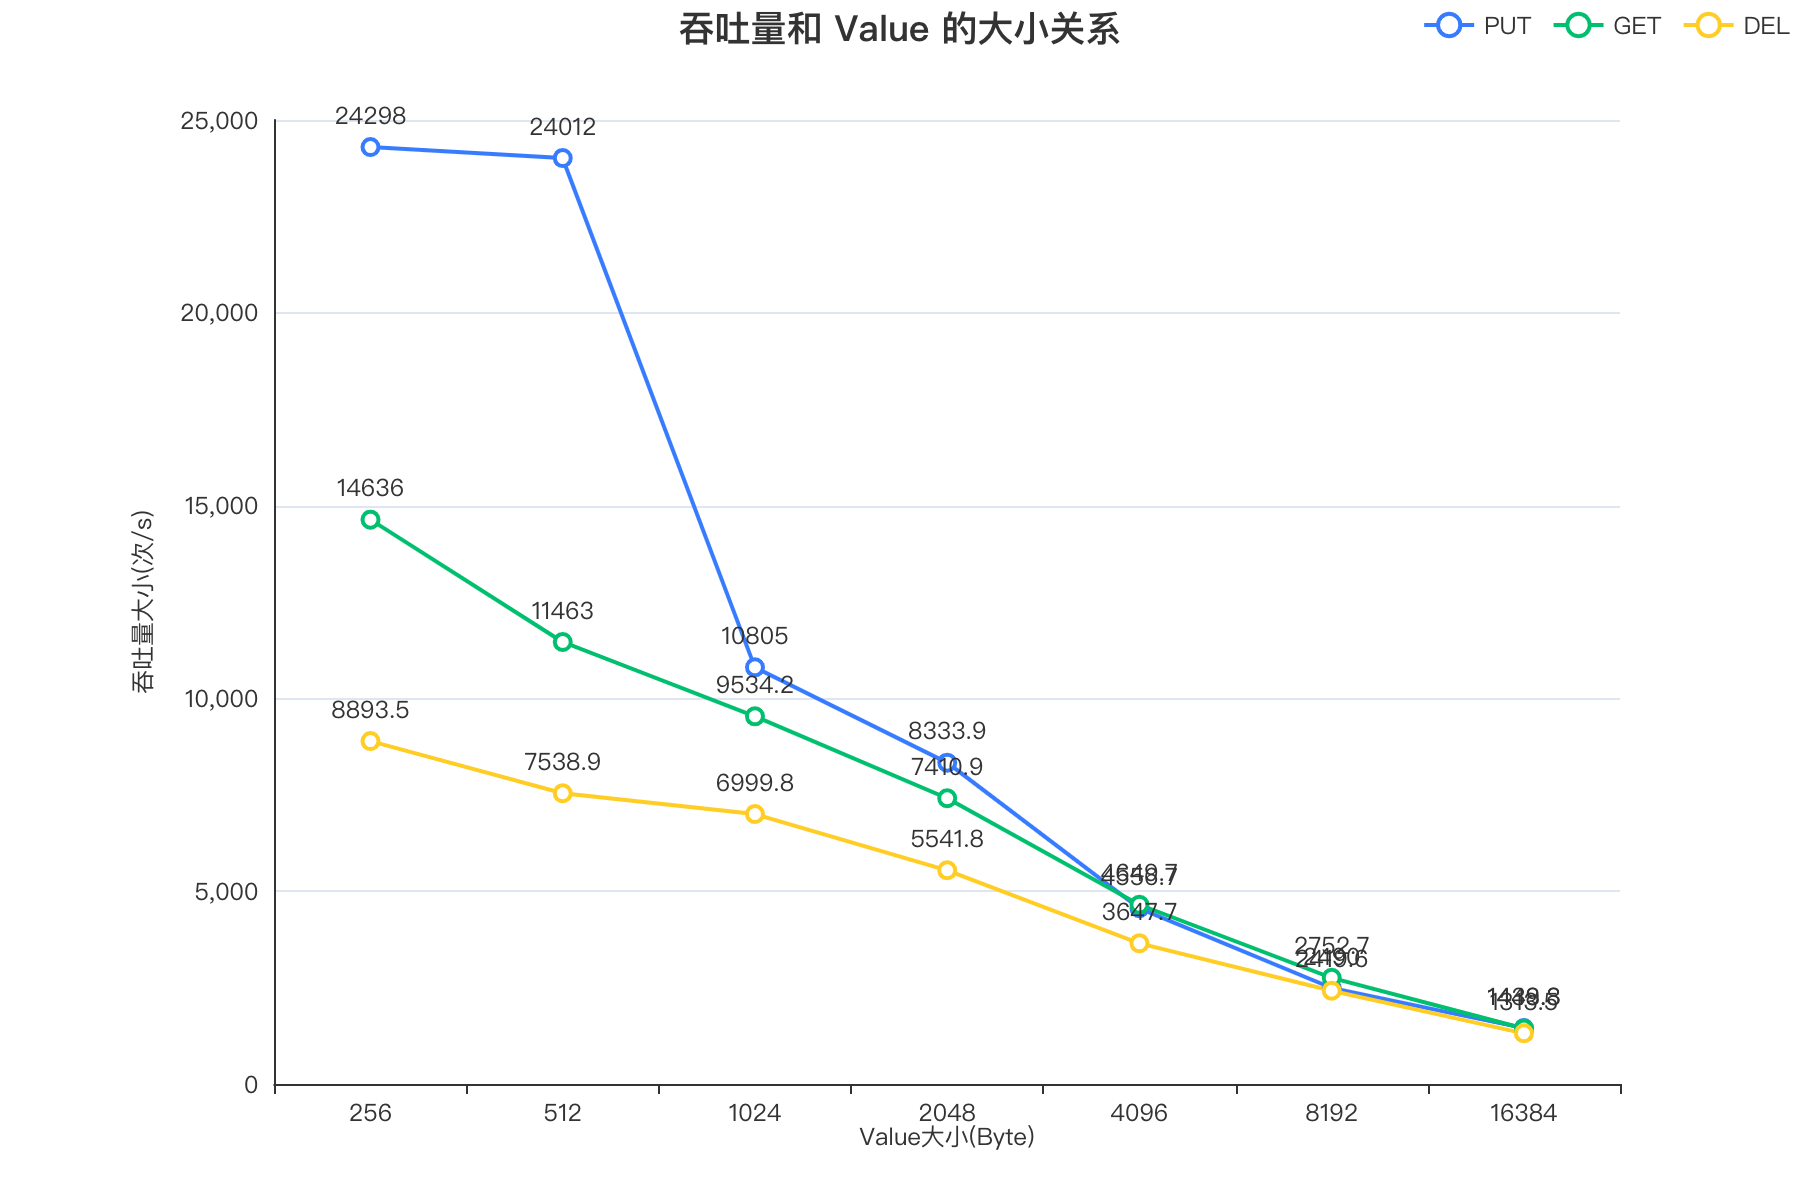
\includegraphics[width=0.98\textwidth]{Image/吞吐量和 Value 的大小关系 (部分).png}
  \caption{吞吐量和 Value 的大小关系(部分)}
  \label{fig:吞吐量和 Value 的大小关系(部分)}
\end{figure}


\subsubsection{索引缓存与Bloom Filter的效果测试}
对比下面三种情况GET操作的平均时延,对比参数为:Value的大小为10240Byte,插入的次数为$1024 \times 16$。对比结果如下
\begin{enumerate}
    \item 内存中没有缓存SSTable的任何信息,从磁盘中访问SSTable的索引,在找到offset之后读取数据
    \item 内存中只缓存了SSTable的索引信息,通过二分查找从SSTable的索引中找到offset,并在磁盘中读取对应的值
    \item 内存中缓存SSTable的Bloom Filter和索引,先通过Bloom Filter判断一个键值是否可能在一个SSTable中,如果存在再利用二分查找,否则直接查看下一个SSTable的索引
\end{enumerate}

\begin{table}[h]
  \centering
  \newcolumntype{Y}{>{\centering\arraybackslash}X}
  \makebox[\textwidth]{
  \begin{tabularx}{\linewidth}{|Y|Y|Y|Y|}
    \hline
        缓存策略 & PUT(s)  &  GET(s) & DEL(s)  \\
    \hline
        无缓存 & $2.0309\times 10^{3}$ & $1.2968\times 10^{3}$ & $1.2961\times 10^{3}$ \\
    \hline
        缓存索引 & $2.0218\times 10^{3}$ & $1.2870\times 10^{3}$ & $1.2916\times 10^{3}$ \\
    \hline
        全部缓存 & $2.0139\times 10^{3}$ & $1.3063\times 10^{3}$ & $1.2994\times 10^{3}$ \\
    \hline
  \end{tabularx}}
  \caption{吞吐量和缓存策略的关系}
\end{table}

关于这个结果,我们关注的是GET操作的吞吐量。可以看到不缓存任何数据、缓存索引、缓存索引和BF过滤器的吞吐量是逐渐递增的,这也是符合我们的预期。


\subsubsection{Compaction的影响}
不断插入数据的情况下,统计每秒钟处理的PUT请求个数(即吞吐量),并绘制其随时间变化的折线图。参数为:Value的大小为10240Byte,插入的次数为$1024 \times 16$。结果如下所示:

\begin{figure}[h!]
  \centering
  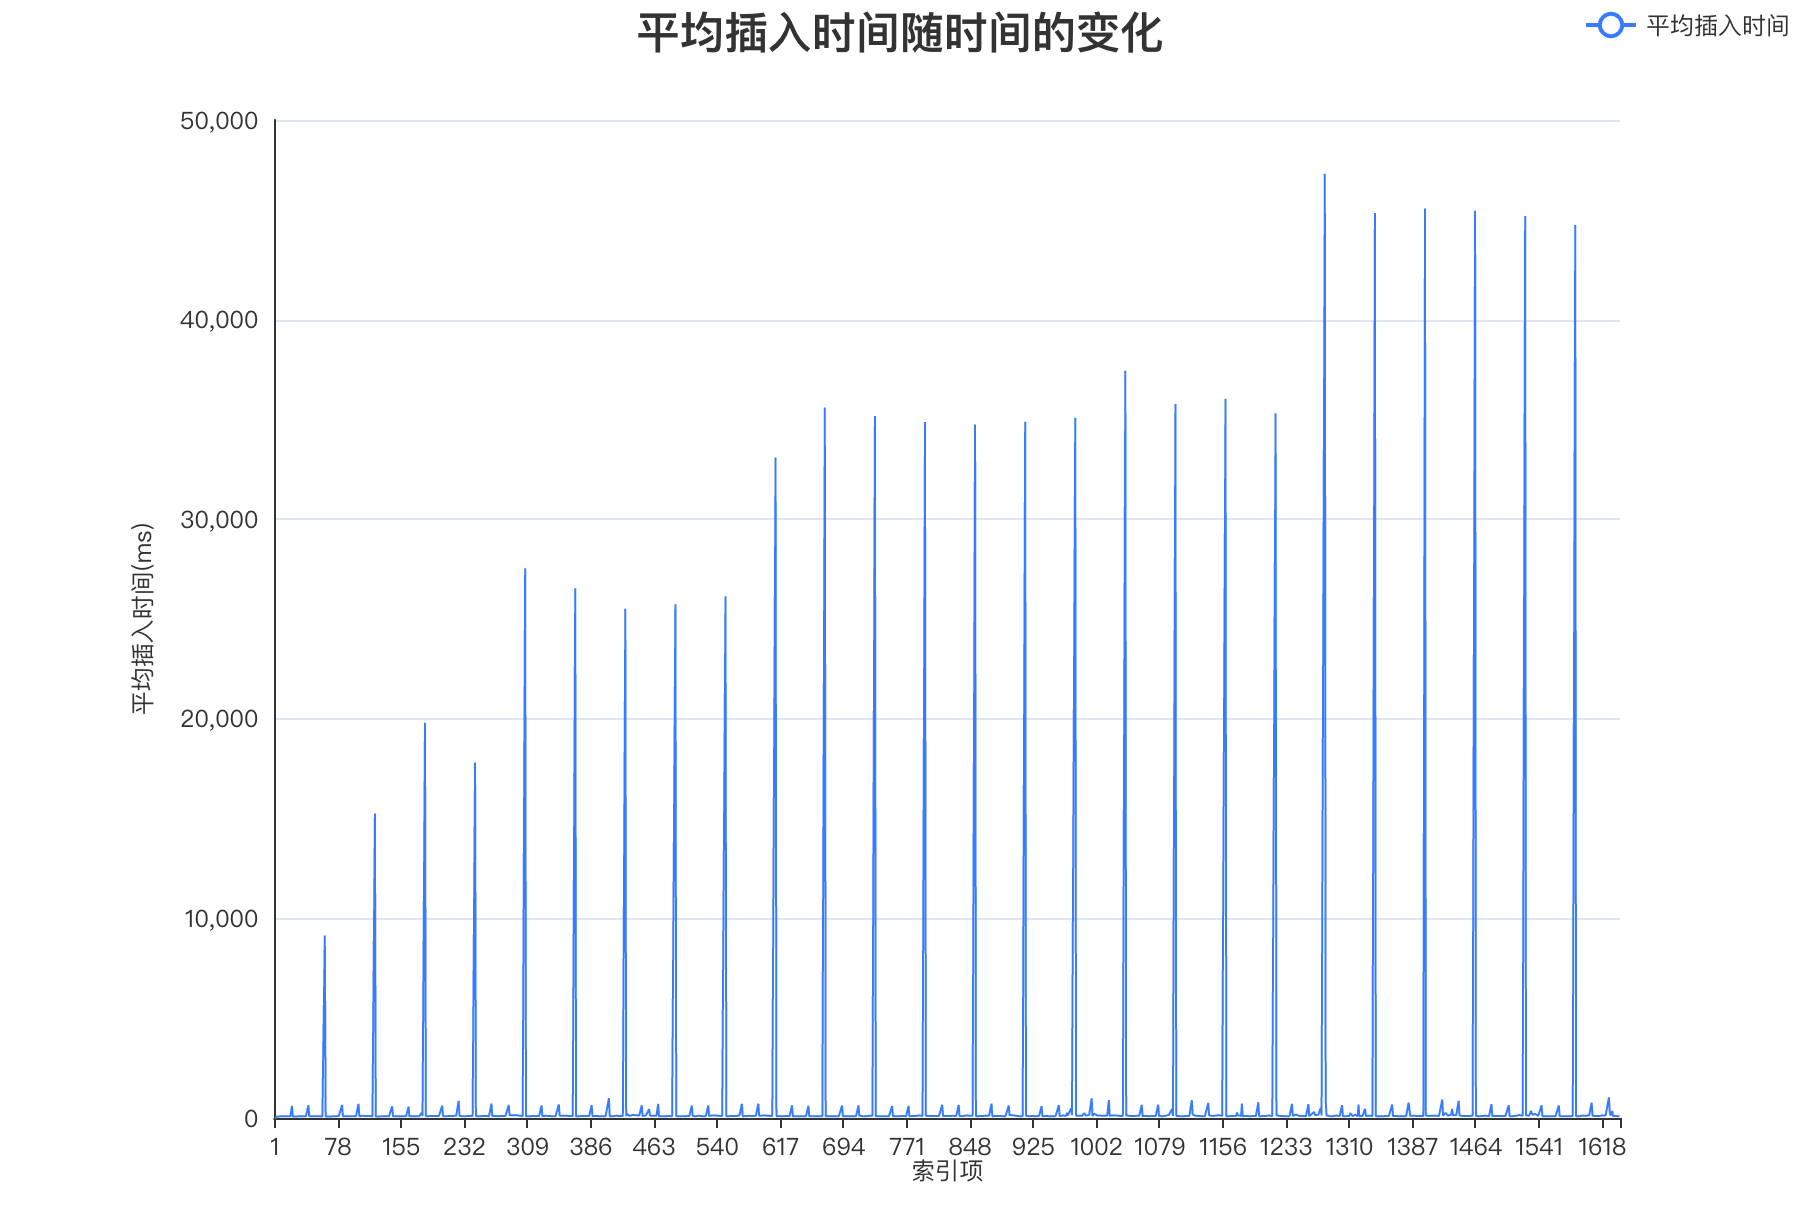
\includegraphics[width=0.98\textwidth]{Image/平均插入时间随时间的变化.png}
  \caption{平均插入时间随时间的变化}
  \label{fig:平均插入时间随时间的变化}
\end{figure}

\begin{figure}[h!]
  \centering
  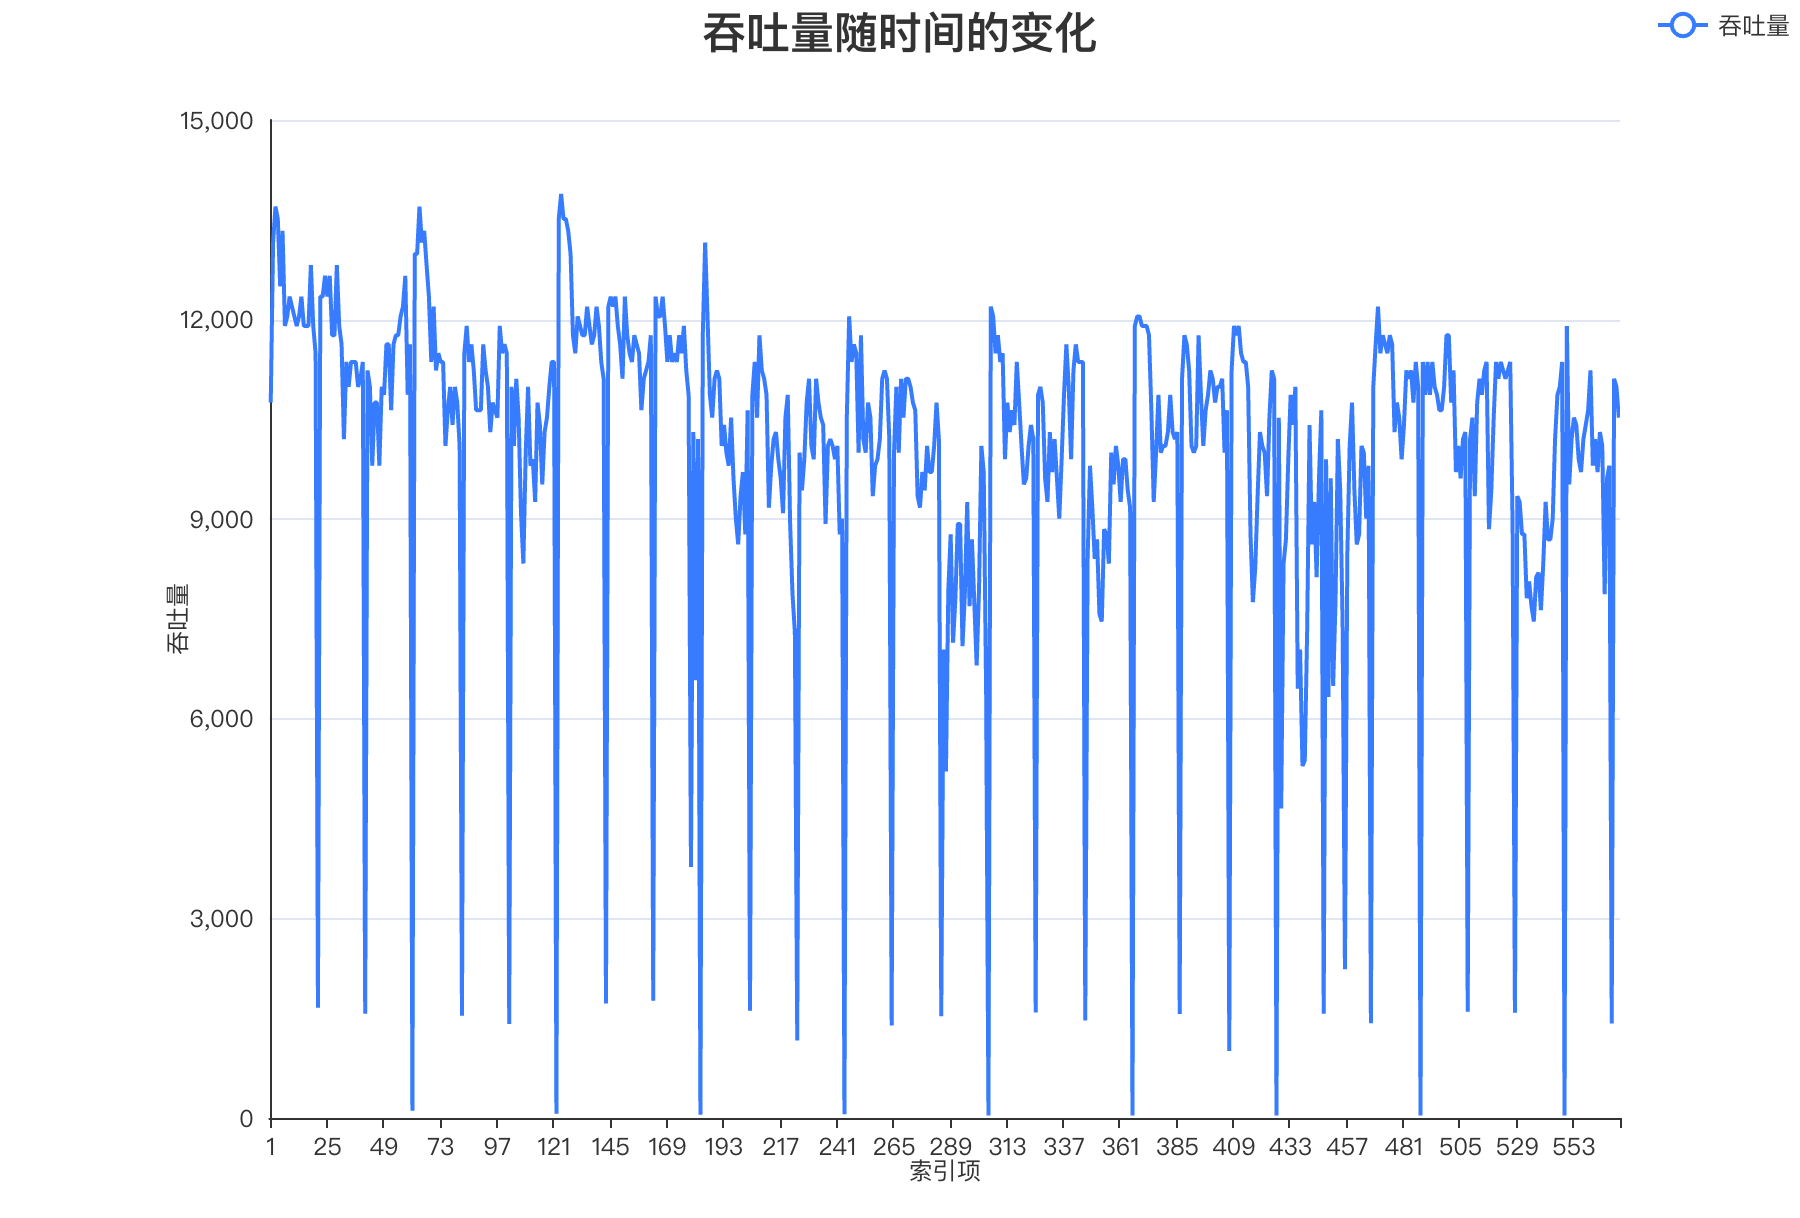
\includegraphics[width=0.98\textwidth]{Image/吞吐量随时间的变化.png}
  \caption{PUT吞吐量随时间的变化}
  \label{fig:吞吐量随时间的变化}
\end{figure}
观察上面两个图,可以看到Merge归并对于时间的影响是突发性的。平均插入时间增加了几乎几百身上几千倍。由于观察吞吐量的效果可能不是太好,观察平均插入时间可能更合适。


\subsubsection{Level配置的影响}
保持测试参数不变:Value的大小为10240Byte,插入的次数为$1024 \times 16$。改变Tiring的层数(从Level0依次开始改变)

\begin{table}[h]
  \centering
  \newcolumntype{Y}{>{\centering\arraybackslash}X}
  \makebox[\textwidth]{
  \begin{tabularx}{\linewidth}{|Y|Y|Y|Y|}
    \hline
        Tiring层数 & PUT(s)  &  GET(s) & DEL(s)  \\
    \hline
        1 & $1.7048\times 10^{3}$ & $1.3489\times 10^{3}$ & $1.2249\times 10^{3}$ \\
    \hline
        2 & $1.6822\times 10^{3}$ & $1.2773\times 10^{3}$ & $1.1883\times 10^{3}$ \\
    \hline
        3  & $1.5895\times 10^{3}$ & $1.2723\times 10^{3}$ & $1.1887\times 10^{3}$ \\
    \hline
        4 & $1.5265\times 10^{3}$ & $1.1971\times 10^{3}$ & $1.1429\times 10^{3}$ \\
    \hline  
        5 & $1.4958\times 10^{3}$ & $1.1737\times 10^{3}$ & $1.1127\times 10^{3}$ \\
    \hline
  \end{tabularx}}
  \caption{吞吐量和Leveling层策略的关系}
\end{table}

基于此表格可以发现,Leveling层数越多,吞吐量越小,所以最佳的配置是:\textbf{仅仅Level-0是Tiering,其余全部是Leveling}。这种状态下吞吐量最大

\section{结论}
基于本次项目的实验和数据,可以得出以下结论:

\begin{itemize}
    \item [(1)] 操作延迟会随着数据量的增大而递增,并且在发生从内存表空间写满时,出现操作延迟突跃现象。
    \item [(2)] 
    配置层策略的时候,推荐配置level-0为Tiering,其余全部都是Leveling,这样的效率最高。
    \item [(3)] 
    在发生Merge的时候,吞吐量会大幅度下降,平均插入时间大大延长。
\end{itemize}


\section{致谢}

特别感谢:语雀文档(yuque.com)为本文的绘图提供的强大支持!

特别感谢:SPASS(spsspro.com)为本论文数据可视化的强大支持!

特别感谢:Github(github.com)提供强大的代码托管和版本管理平台!

特别感谢:VSCode(code.visualstudio.com)作为本项目开发的开发工具!

特别感谢:Overleaf@SJTU(latex.sjtu.edu.cn)提供论文撰写的在线工具!

特别感谢:WilliamX1(github.com/WilliamX1)的文档,为我修复4744Bug提供了灵感

\section{收获和可能的问题}

\subsection{收获与问题}
我从头开始完成整个Project项目(包括附加WAL/Scan、各种测试)功能大概花费了一周时间,整个项目难度不大(对个人而言,也可能是因为之前积累的经验还算比较丰富),但是完成下来的过程还是踩了不少的坑。例如我是万万没有想到相同key相同时间戳的情况,我一直认为同一个时间戳一定是同时被写入sst文件的,但是我忽略了一个情况,那就是归并的时候可能把小的时间戳提升到大的时间戳,这样会带来问题。我花费了两天的时间探索这个Bug的存在,以至于我愿意称之为\textbf{4744号Bug},关于我是如何解开这个谜团的Debug过程,我也分享到了我Commit的评论区,\href{https://github.com/Musicminion/2022-2023-2-Advanced-Data-Structure/commit/788e97b823a08bb03a8ae1b3aa83fd1b530323b1#commitcomment-104192045}{\underline{4744号deBug经历。}}

最后我还愿意分享一下我在做这个项目中的思考的问题。这些问题如果可以思考到位,我觉得这个项目的收货才是最值得的。也希望这些思路能够给后来人以帮助!

\begin{itemize}
    \item [1)] \textbf{问题:当项目出现测试数据不通过的时候,该如何Debug?}
    
    \textbf{回答}:这个项目的架构算稍微有一些复杂的,从顶层的kv-store,到下面的跳表、sstable文件读写模块,都有可能出现Bug。从根源来说,应该写完一个组件就立即测试,尽早发现问题。如果最后仍然出现测试数据不通过的时候,为了更快的定位,首先需要确定:是否是Merge阶段出现问题(因为Merge是最复杂的步骤),解决方式是\textbf{把第0层的文件限制设为无穷大},也就是直接修改default配置文件,这样就不会触发归并的限制。如果这样修改之后测试全部通过,那就是归并的问题,否则是其他模块的问题。
    
    另外一种debug方式是\textbf{数据跟踪},例如第i个测试数据出现问题,我就在归并或者查找的过程,用一个if判断是否查找的是这个key,如果是的话就打印出相关的调试信息。这样可以更快的定位到问题。
    
    \item [2)] \textbf{问题:为什么会出现相同key相同时间戳的情况、为什么选择楼层小的?是否可能相同时间戳的key出现在同一楼层的不同文件里面?}
    
    \textbf{回答}:在merge的时候,会把小的时间戳的sst文件变成一个大的时间戳的文件,这个本质是导致了数据的丢失的(从直觉上来说),也埋下了很多隐患。那么,为什么相同key相同时间戳,level小的楼层里面,就是我们要找的呢?根据我们的归并规则,LevelingX层的选择,优先选择的是小的时间戳的sst文件(这些文件会被下沉到X+1层),剩下的时间戳就是较大的时间戳,也就是说,X+1层的文件的时间戳一定小于或者等于X层的文件的时间戳。(\href{https://github.com/Musicminion/2022-2023-2-Advanced-Data-Structure/commit/63726308274f04282bbb7ae7b08928f4a87f2263#commitcomment-104586158}{\underline{Commit补充:4744号deBug根源分析}})

\end{itemize}

\subsection{WAL和SCAN的实现}

关于WAL的实现机制,我是放在MemTable这个类里面的。这可能和我最初的文件读写放在底层组件的构想有一点差异,但是最佳的方法确实是放在MemTable中。每次启动的时候,MemTable需要检测是否有WAL文件存在,如果存在就需要恢复WAL的数据,依次执行插入或是删除操作(注意!这个时候插入或者删除不能写日志,否则就会死循环,所以通过私有的插入函数实现,此外插入或者删除需要更新当前内存表的数据大小),而MemTable对外暴露的接口插入和删除首先就需要写日志。

关于Scan的实现机制,稍微比较复杂,因为删除的本质是插入了一个特殊字符,所以在扫描到删除符号的处理\textbf{比较复杂,需要分情况考虑},尤其是当时间戳较大的删除标记出现的时候需要覆盖之前的(而不是查找的时候直接忽略删除标记)。

扫描分两个步骤,先扫描sst文件,再扫描内存表。扫描sst文件时候,先从最底层sst文件开始扫描,然后往上层。这是因为相同key、相同时间戳,优先保留上层的数据,所以采取层方面倒序,这样新的数据就可以覆盖旧的数据。对于每个sst文件的扫描,还是类似二分法的查找机制,找到扫描起点key在sst文件的位置,然后往后扫描(当然需要检查扫描的key小于key2)。\textbf{如果遇到删除标记,需要清空当前key之前扫描到的结果},否则会出现幻读(读取到已经删除的数据)

\subsection{建议}
当然,关于这个Project我也有一些建议:
\begin{itemize}
    \item [1)] 评测程序希望有更强大复杂的评测脚本,例如通过多进程fork来进行持久化判断的。同时评测程序对于错误的输出\textbf{很不友好},会输出长度将近几千个,且字母都是一样的Value的值,实际上只需要输出value的前十个字母即可了。
    \item [2)] 文档希望更详细(当然我觉得适度留白恰恰增加了我的思维能力,debug能力)
    
    \item [3)] 时间戳的设计思路理论上没有问题(我起初认为Merge阶段时间戳选择最大会带来后续问题,实际上不会,具体的证明我写在了\href{https://github.com/Musicminion/2022-2023-2-Advanced-Data-Structure/commit/63726308274f04282bbb7ae7b08928f4a87f2263#commitcomment-104587485}{\underline{Commit:证明归并时间戳不会丢失数据}}),但是在实现和维护时间戳的时候复杂程度大大增加,可以说(牺牲了算法的易理解性、复杂性换来了空间的节省),尤其是归并的时候会修改一些文件的时间戳,这个我认为是丢失了一些信息的。反而对于一个真实的存储系统来说不太好。如果每个数据维护一个时间戳的话,可能是一个更简单更好的选择,尽管可能会增加一些文件的大小。 
    
    \item [4)] 关于这个kv-store系统,一个问题就是删除的数据永远在里面。哪怕我插入10000个数据,再执行删除10000个数据,sst文件里面依然存在这些数据插入和删除的记录,冗余数据的处理可能还需要做进一步的优化。
\end{itemize}

\section{参考文献}
\begin{itemize}
    \item [1)] 项目说明文档kv-store
    \item [2)] 文件读写样例:https://blog.csdn.net/hcf999/article/details/77864456
\end{itemize}


\end{document}
